\section{Backgrounds evaluation}
\label{sec:backgrounds}
% ---- ---- ---- ---- ---- ---- ---- ---- ---- ---- ---- ---- ---- ---- ---- ---- ---- ---- ---- ---- ---- ---- ----


\subsection{W + jets}
% .... .... .... .... .... .... .... .... .... .... .... .... .... .... .... .... .... .... .... .... .... .... ....

The W+jets background is the dominant contamination in the signal region.
Several methods are foreseen to measure this background from data, 
as the shape of the four-body mass is not well described by the simulation below 400~GeV, 
as can be seen in figure~\ref{fig:M4body_afterPreselections}.


\subsection{QCD}
% .... .... .... .... .... .... .... .... .... .... .... .... .... .... .... .... .... .... .... .... .... .... ....

The residual contribution of the QCD background after the selections listed in section~\ref{sec:H0j_selections_cut}
is at the level of 5\% for electrons, and considered negligible for muons.

To estimate this residual contribution for electons, 
we measure the QCD \MET shape from data in a QCD enriched sample
and use this shape to fit the \MET distribution in the signal phase space, 
but the \MET requirement itself. 

The QCD enriched sample is built by inverting the isolation on the electron in the final state, 
by requiring the relative isolation to be between 0.15 and 0.3. The composition of events in the 
constrol region is shown in table \ref{tab:invIsoYields}.

\begin{table}[htb]
  \begin{center}
  \begin{tabular}{c|c|c|c}
  \hline
        & QCD  & W+jets & Other \\
  \hline
  scaled events (1 fb$^{-1}$)    & \scriptsize{$1680.46$} & \scriptsize{$1.49$} & \scriptsize{$157.59$} \\
  
  fraction (\%)                & \scriptsize{$91.35$} & \scriptsize{$8.57$} & \scriptsize{$0.08$} \\
  \hline
  \end{tabular}
  \end{center}
  \caption{Expected number of events in the Anti-Iso control region. The yields are shown for the two main processes
           and the residual contributions are summed up together.}
  \label{tab:invIsoYields}
\end{table}

To select this control region the isolation distribtion variable has been studied from MC simulation (fig \ref{fig:bkg_QCD_IsoShape})
and the cuts have been tuned so that the contribution of the QCD exceeds the $90\%$ of the total.

% as defined in table~\ref{tab:invIsoCuts}.
%\begin{table}[htb]
%  \begin{center}
%  \begin{tabular}{l|c}
%  \hline
%  lepton    &   inverted isolation \\
%  \hline
%  electons  &                      \\ 
%  muons     &                      \\ 
%  \hline
%  \end{tabular}
%  \caption{}
%  \label{tab:invIsoCuts}
%  \end{center}
%\end{table}%
%

Figure~\ref{fig:bkg_QCD_METMCShape} shows the \MET distribution in the isolated and non-isolated regions, 
as seen in the simulation, for the QCD events; Anti-Iso data are superimposed. 
The compatibility of the QCD shapes \footnote{The Kolmogorov-Smirnov test between the MC QCD Iso and Anti-Iso gives 0.51} 
in the two regions suggest the possibility to use as a template function for the \MET distribution fit the one taken 
from the non Isolated data. 

\begin{figure}[h]
  \begin{center}
    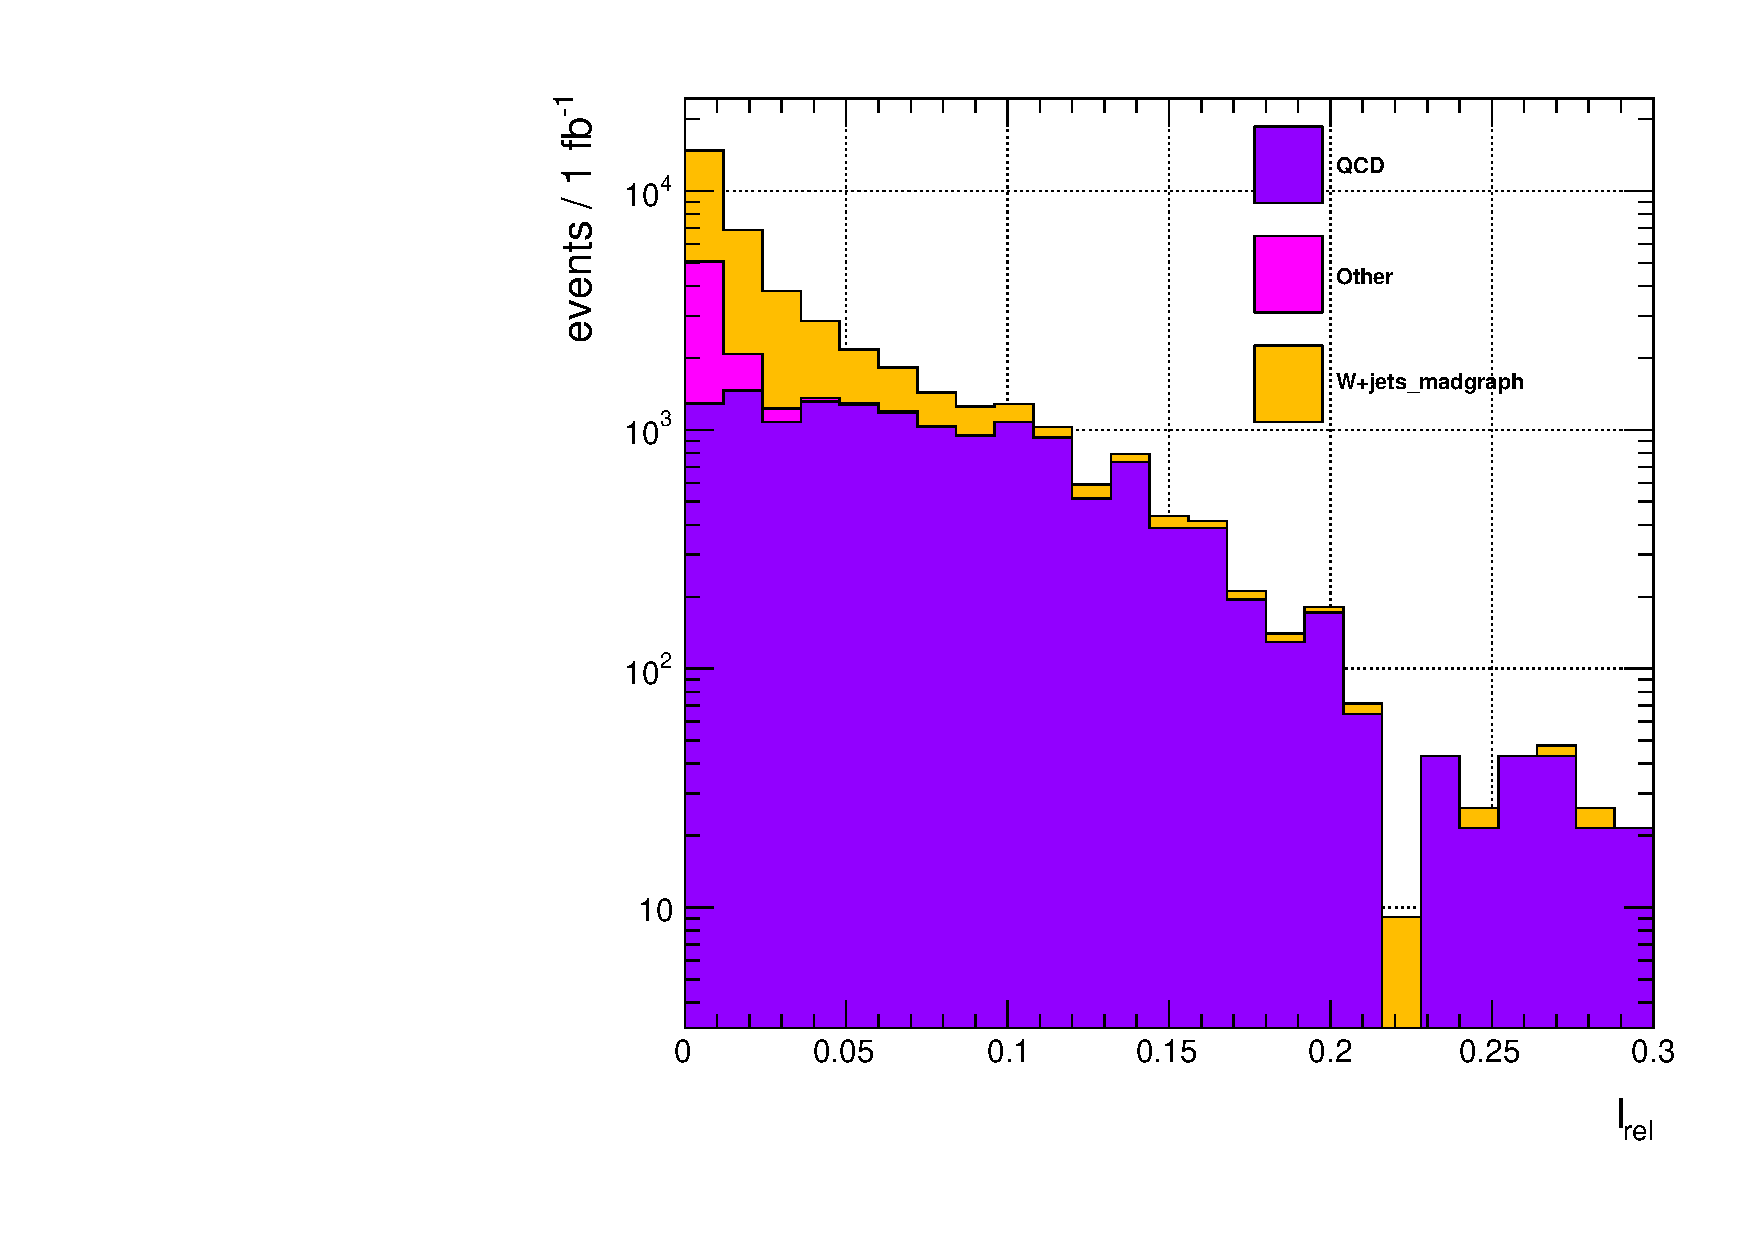
\includegraphics[width=0.45\textwidth]{plots/bkg_IsoStack.pdf}
    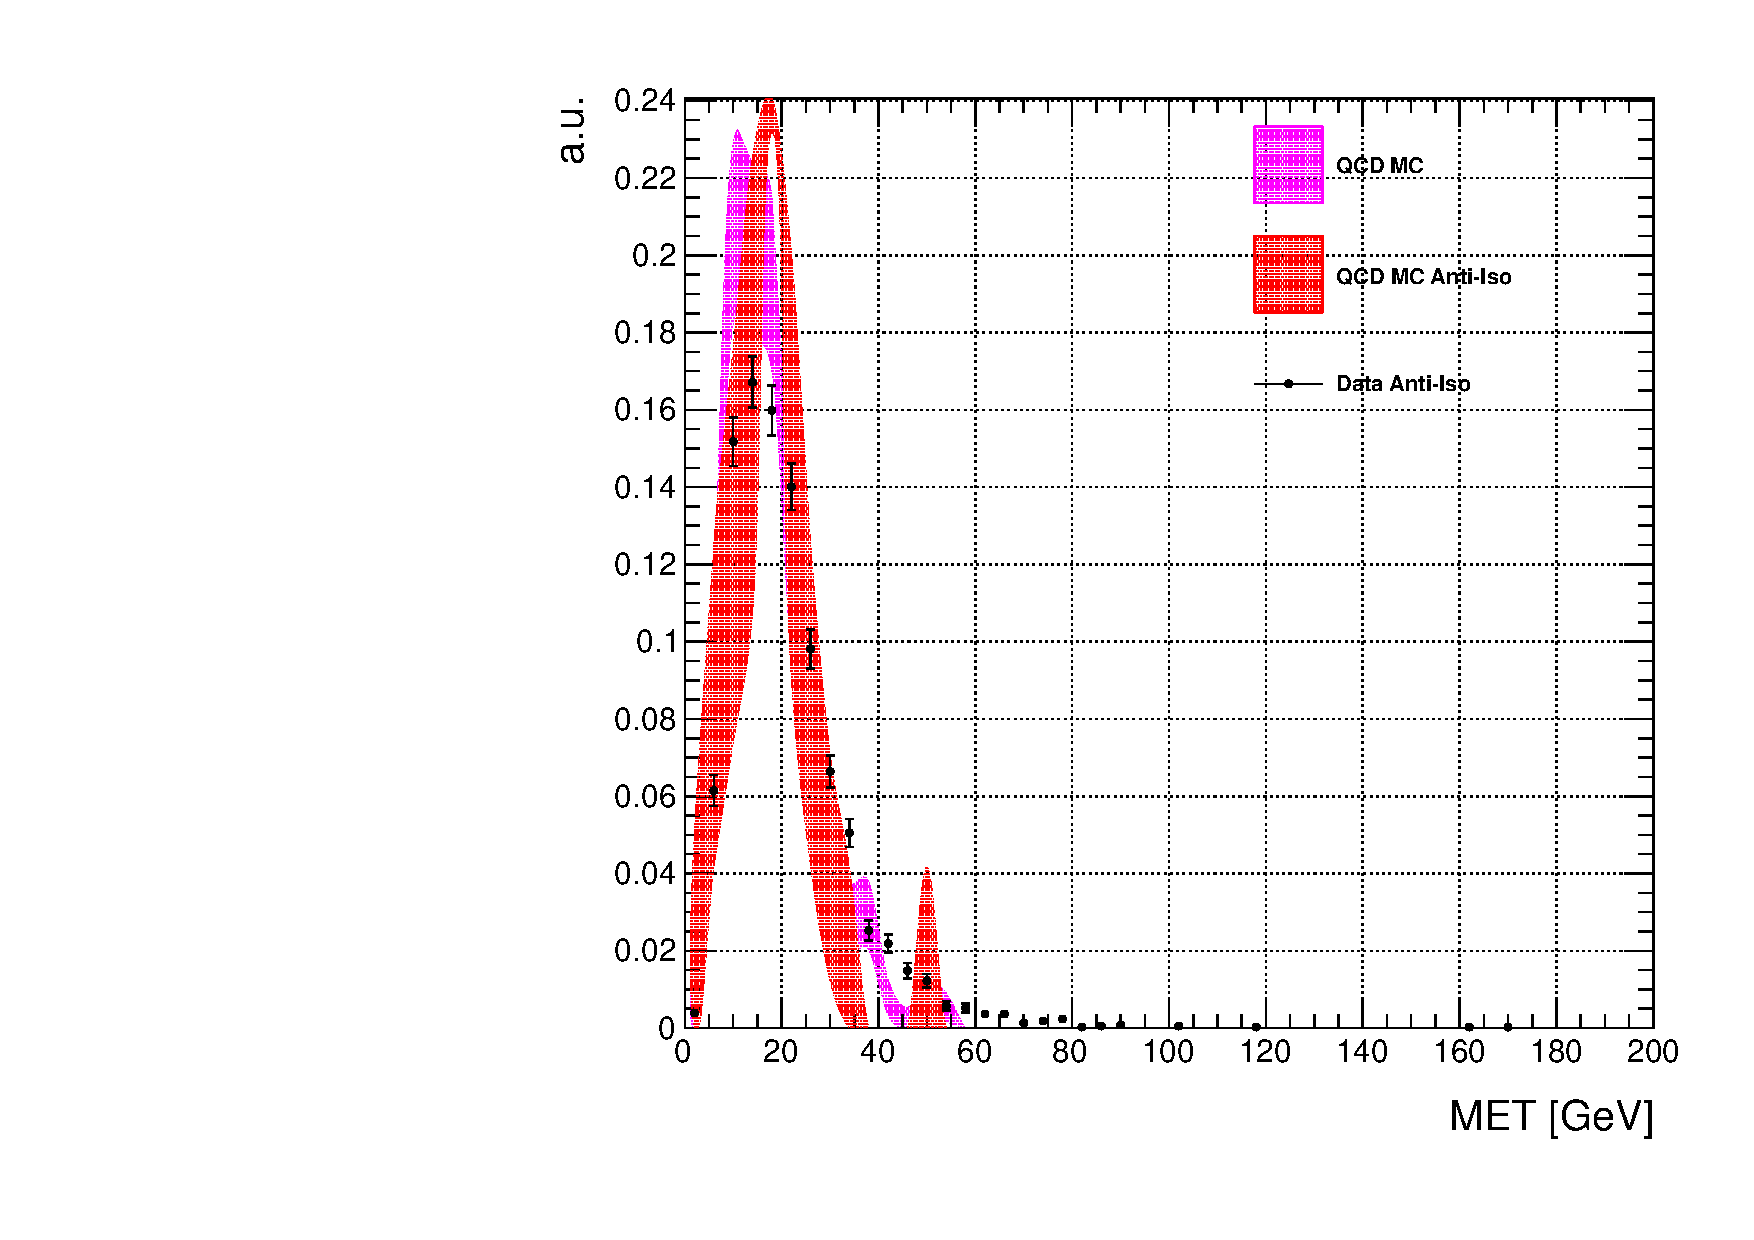
\includegraphics[width=0.45\textwidth]{plots/bkg_IsoShape.pdf}
    \caption{The $I_{rel}$ distribution (left) for the QCD, w+jets and other backgrounds from MC simulation. 
             Events are scaled to $1\ fb^{-1}$. \MET distributions (right) for the QCD in the Iso and Anti-Iso region 
             from MC simulations. Bands take into account statistical MC poissonian statistical fluctuation.
             Data in the control region for $950 pb^{-1}$ are superimposed.}
  \label{fig:bkg_QCD_IsoShape}
  \end{center}
\end{figure}

The fit of the \MET shape in the isolated region is shown in figure~\ref{fig:bkg_QCD_METStack}.
The fit is perfomed by maximizing a binned likelihood function, where all the PDFs are taken 
from MC, except the QCD that is obtained by inverting the isolation cut on the $950\ pb^{-1}$ 
sample of electron data. The free parameters of the fit are the QCD normalization and a global
normalization of the other backgrounds. The relative normalization of non-QCD events are taken
from MC.

To get the number of QCD events in the signal region, the fit distribution of the QCD events is integrated
in the $[30,\ +\infty)$ \MET range and the results are reported in table \ref{tab:bkg_QCD_DDYields}.

\begin{table}[htb]
  \begin{center}
  \begin{tabular}{c|c|c}
  \hline
         channel  & QCD MC expectation ($1\ fb^{-1}$) & QCD DD estimation ($1\ fb^{-1}$) \\
  \hline
  $e$    & \scriptsize{$(1.4\pm0.3)\cdot10^3$} & \scriptsize{$(3.3\pm0.1)\cdot10^3$}  \\
  \hline
  \end{tabular}
  \end{center}
  \caption{Expected number of QCD events for $1\ fb^{-1}$. The yields are shown for the pure
           MC expectation and the DD correction. Quoted errors take into account the MC statistics
           and the fit error respectively.}
  \label{tab:bkg_QCD_DDYields}
\end{table}
  
The error on the DD correction is taken from the likelihood function width. The method works with the first fraction of 
data sample since in that period the exploited triggers were not using any cut on the \MET; to get 
the contribution for the whole statistics we scale the results linearly with the luminosity.

To get the contribution of the QCD in the signal region defined in section \ref{sec:H0j_selections_intro} 
we scale the contribution evaluated with the presented method with the selection efficiency obtained
from the MC study.

\begin{figure}[h]
  \begin{center}
    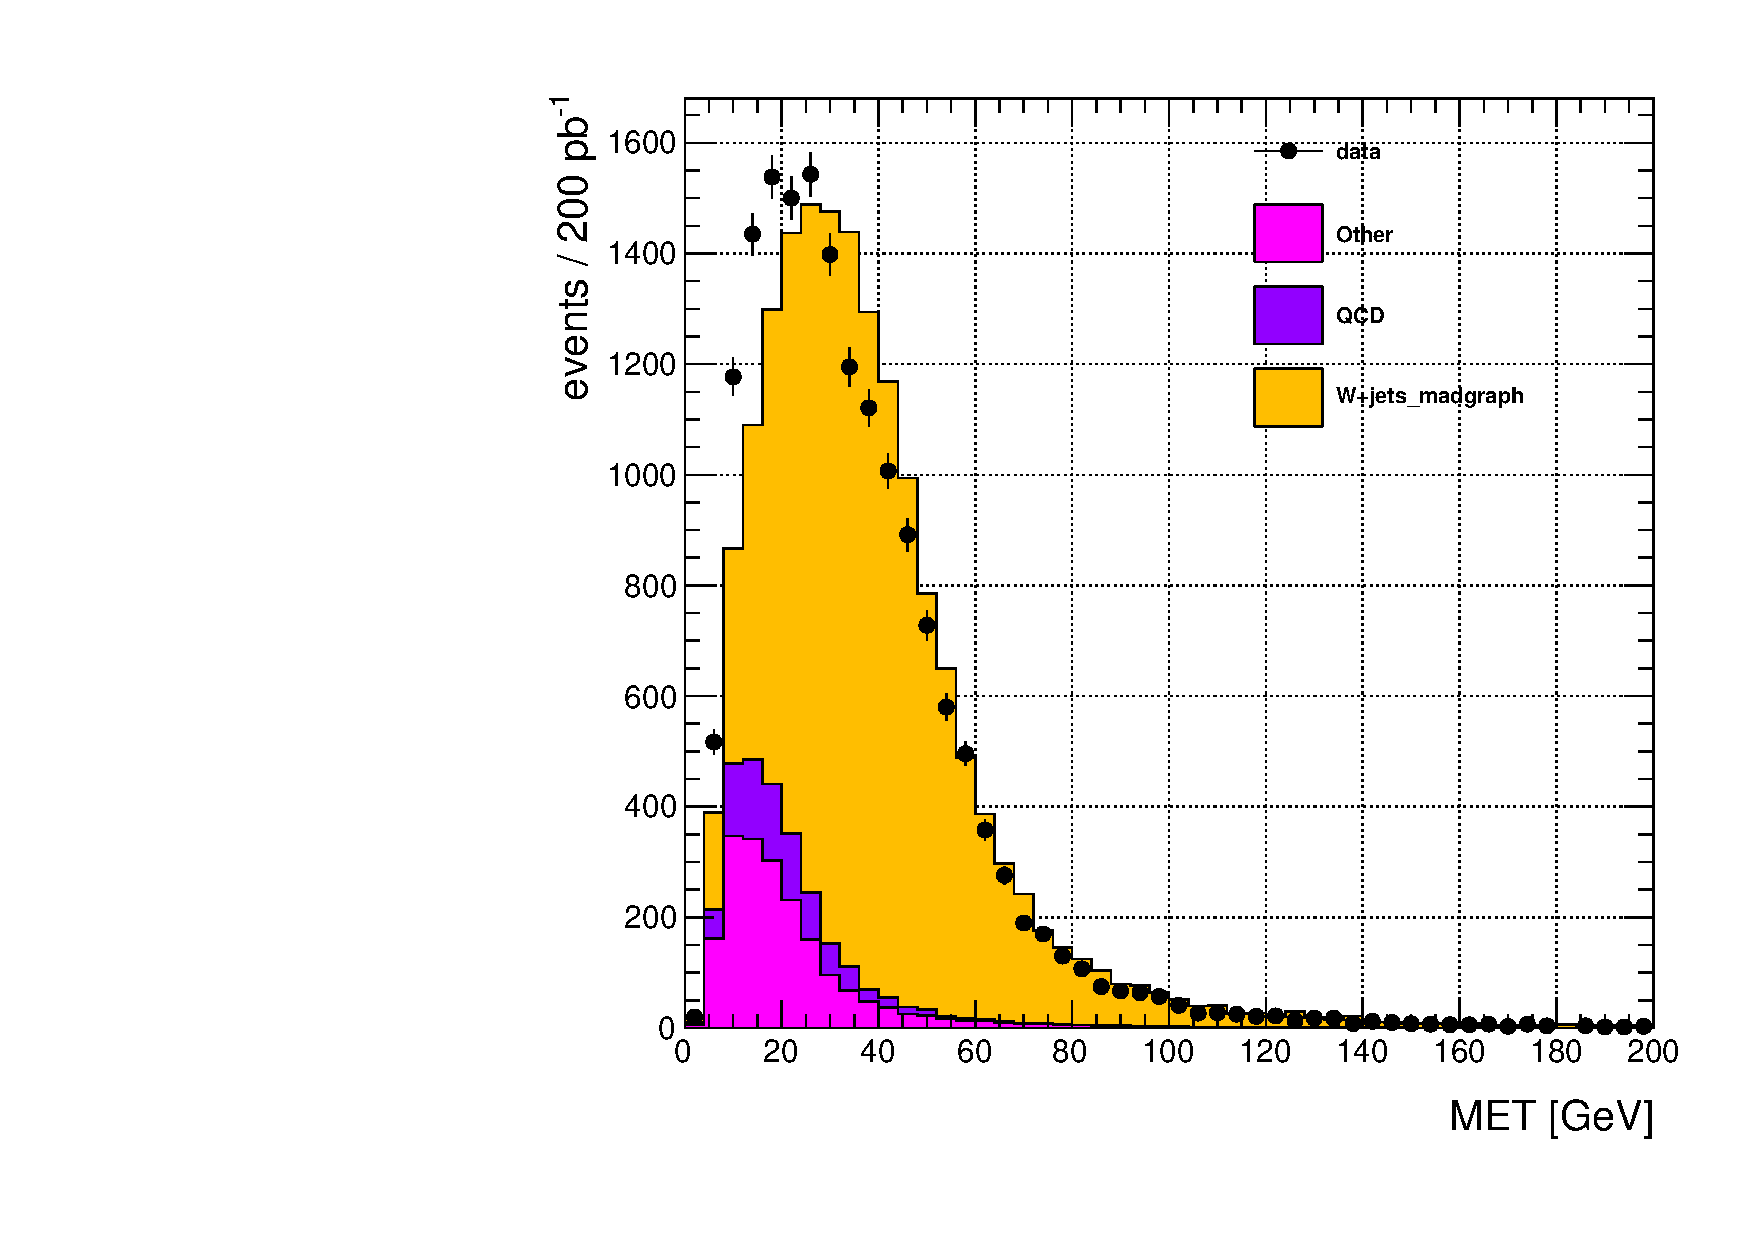
\includegraphics[width=0.45\textwidth]{plots/bkg_METStack_NoFit.pdf}
    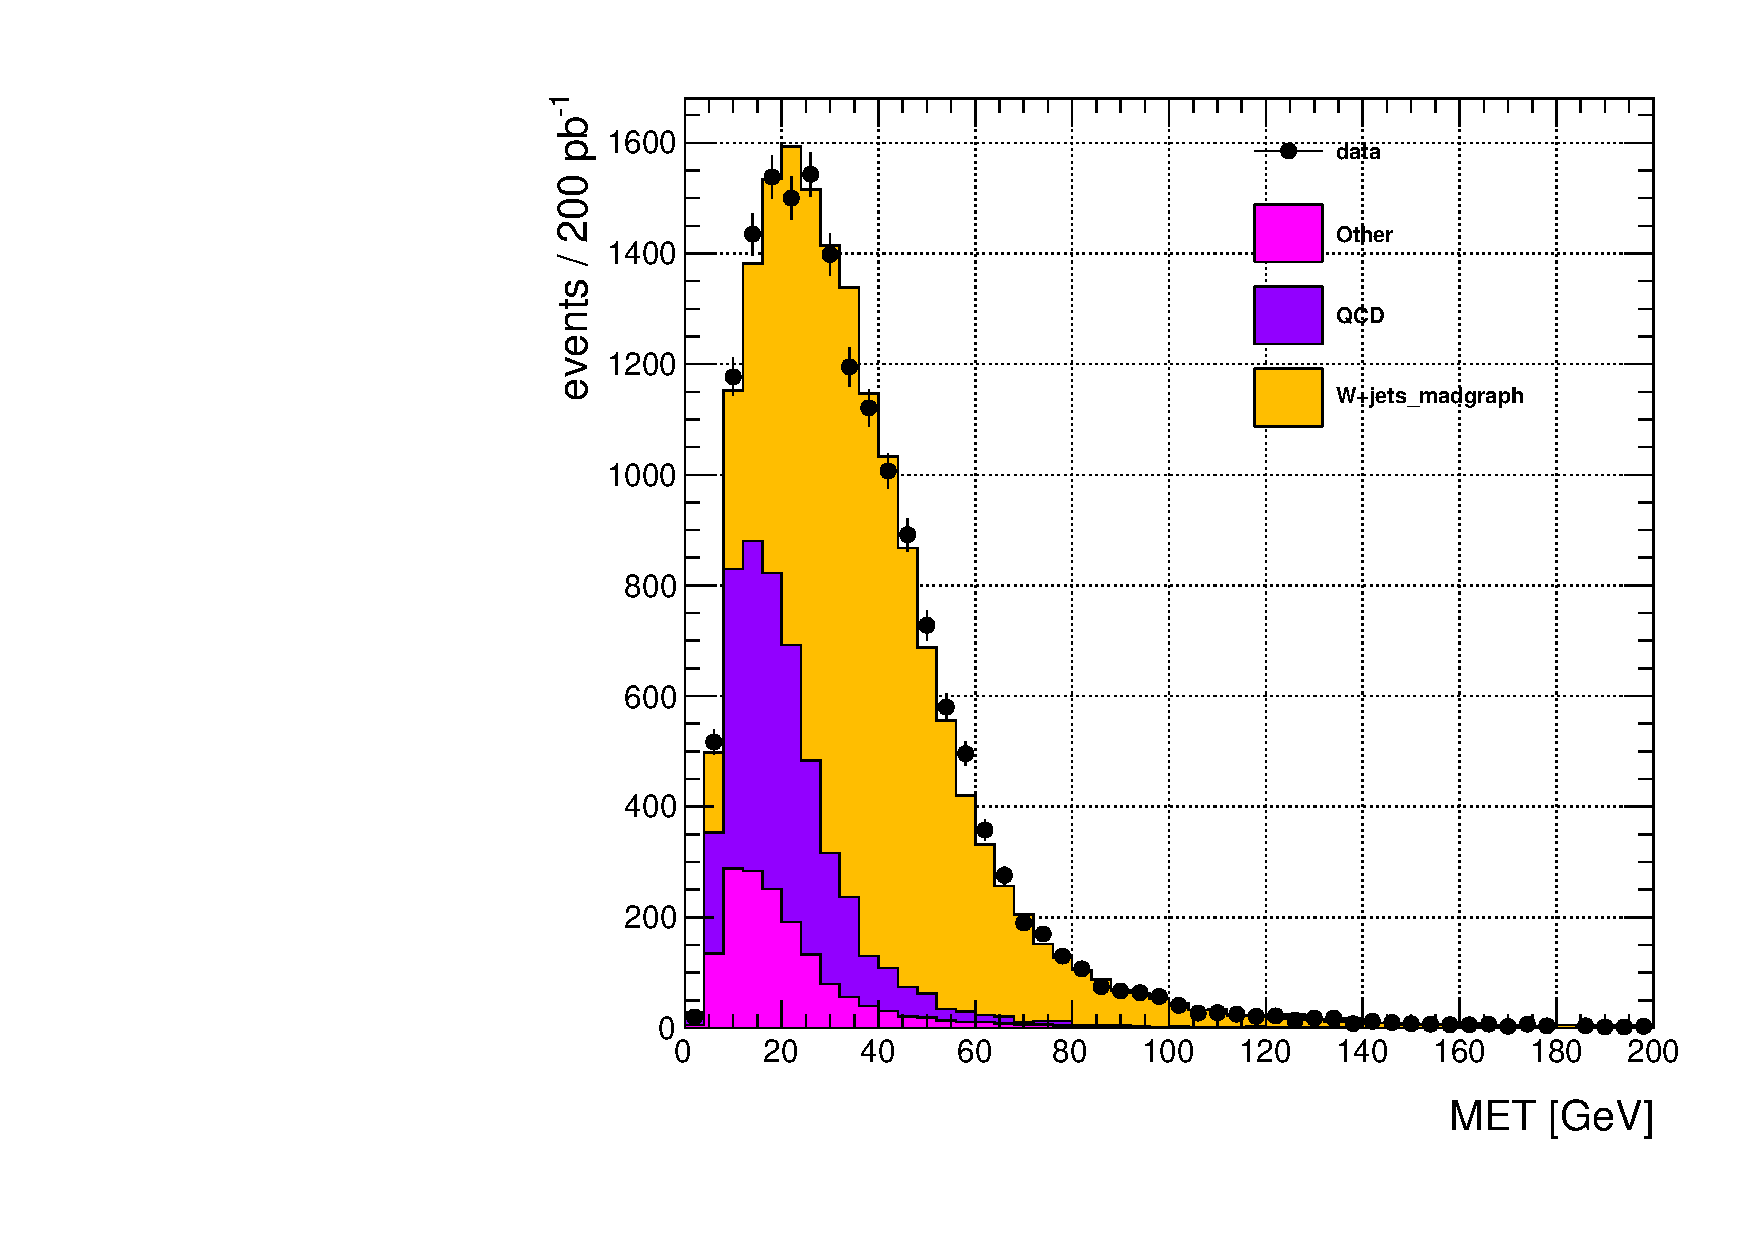
\includegraphics[width=0.45\textwidth]{plots/bkg_METStack.pdf}
    \caption{The DATA-MC comparison before (left) and after (right) the fit of 
             the \MET in the isolated region for the electrons. 
             The QCD shape is extracted from the non-isolated region.  
             while other processes shapes are taken from MC. MC is normalized to DATA.}
  \label{fig:bkg_QCD_METStack}
  \end{center}
\end{figure}

The contribution due to muon fakes is expected to be subleading with respect the electrons one, 
and considered negligible.
Figure \ref~{fig:blablabla} shows the distribution of events where leptons do not pass anti-isolation 
for muons (left) and electrons (right). \textbf{FIXME}

\subsection{ttbar}
% .... .... .... .... .... .... .... .... .... .... .... .... .... .... .... .... .... .... .... .... .... .... ....

The ttbar background contribution
is evaluated by using the Monte Carlo prediction of it.

\subsection{other backgrounds}
% .... .... .... .... .... .... .... .... .... .... .... .... .... .... .... .... .... .... .... .... .... .... ....
